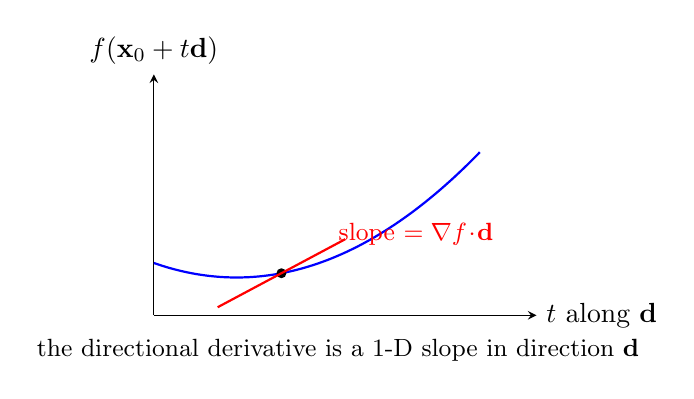
\begin{tikzpicture}[scale=0.9,>=stealth]
\draw[->] (0,0)--(5.4,0) node[right]{$t$ along $\mathbf d$};
\draw[->] (0,0)--(0,3.4) node[above]{$f(\mathbf x_0+t\mathbf d)$};
\draw[domain=0:4.6,smooth,variable=\t,thick,blue] plot (\t,{0.15*(\t-1.5)^2 + 0.1*\t + 0.4});
\fill (1.8,{0.15*0.09 + 0.18 + 0.4}) circle (2pt);
\draw[red,thick] (0.9,{0.5935-0.48})--(2.7,{0.5935+0.48});
\node[red] at (3.7,1.15) {\small slope $=\nabla f\!\cdot\!\mathbf d$};
\node at (2.6,-0.5) {\small the directional derivative is a 1-D slope in direction $\mathbf d$};
\end{tikzpicture}
